%%%%%%%%%%%%%%%%%%%%%%%%%%%%%%%%%%%%%%%%%%%%%%%%%%%%%%%%%%%%%%%%%%%%%%%%%%%
%
%		Relazione del progetto di Design Patterns
%
%				    Nicola Corti - 2014
%
%%%%%%%%%%%%%%%%%%%%%%%%%%%%%%%%%%%%%%%%%%%%%%%%%%%%%%%%%%%%%%%%%%%%%%%%%%%
\documentclass[a4paper,12pt]{article} 
\usepackage{graphicx}
\usepackage{vmargin}
\usepackage[italian]{babel} 
\usepackage[utf8x]{inputenc}
\usepackage{listings}
\usepackage{url}
\usepackage{pdflscape}
\usepackage{tabularx}
\usepackage{hyperref}
\usepackage{amsfonts}
\usepackage[usenames,dvipsnames,svgnames,table]{xcolor}

\usepackage{caption}
\usepackage{subcaption}

\setlength{\parskip}{8pt}

%\usepackage{chngcntr}
%\counterwithin{equation}{subsection}

\renewcommand\lstlistingname{Codice}
\addto\captionsitalian{\renewcommand\figurename{Immagine}}

%\setpapersize{A4}
%\setmarginsrb{15mm}{10mm}{15mm}{10mm}%
%             {0mm}{10mm}{0mm}{10mm}


\definecolor{LightLightGray}{RGB}{241,241,241}

\lstset{
basicstyle=\scriptsize\ttfamily,
keywordstyle=\color{MidnightBlue}\bfseries,
identifierstyle=\color{Black},
commentstyle=\color{Green}\itshape,
stringstyle=\color{Red}\ttfamily,
showstringspaces=false,
%numbers=left, numberstyle=\tiny,
%stepnumber=1, numbersep=10pt,
tabsize=4,
framexleftmargin=5mm, rulesepcolor=\color{LightLightGray},
frame=tb,
backgroundcolor=\color{LightLightGray},
language={Java},
%mathescape=true,
%fontadjust=true,
breaklines=true,breakatwhitespace=true,breakautoindent
}

\title{StarCastle - Esempio di applicazione dei design pattern nella modellazione di un videogioco}
\author{Nicola Corti - 454413 \\Corso di Laurea Magistrale in Informatica - Universit\`a di Pisa}
\date{22 Aprile 2014}

 
\begin{document}
\maketitle

\begin{abstract}
Questa relazione ha lo scopo di illustrare come i design pattern possono essere utilizzati nella modellazione di un software complesso, quale pu\`o essere un videogioco. Gli aspetti da tenere in considerazione sono svariati, dal mantenimento di uno stato consistente, alla gestione degli eventi, delle collisioni, etc\dots{}

Il codice sorgente allegato \`e da considerarsi parte integrante di questa relazione, al fine di permettere una comprensione pi\`u organica di tutti gli aspetti di design ed implementativi.
\end{abstract}

\tableofcontents
\newpage

\section*{Introduzione}
\label{sec:introduzione}

I videogiochi rappresentano forse la categoria di software pi\`u complessi da realizzare, coinvolgendo in un unico progetto svariati aspetti dell'informatica (si pensi al networking, all'intelligenza artificiale o alla gestione dei database).

La realizzazione di un videogioco, se non supportata da un'accurata fase di analisi e di progettazione, pu\`o risultare veramente complessa o addirittura impossibile. Tralasciare la fase di progettazione di un videogioco potrebbe portare a notevoli perdite di tempo o addirittura al fallimento del progetto stesso.

Per questo motivo risulta fondamentale analizzare sotto ogni aspetto il videogioco che si intende realizzare, e progettare ogni classe/interfaccia con la massima accuratezza. In questa fase dello sviluppo i \emph{design pattern} possono essere un strumento valido per risolvere alcune delle problematiche pi\`u comuni e ricorrenti nel campo dello sviluppo di videogiochi.

In particolare in questa relazione mostreremo come i \emph{design pattern} possono essere di supporto nella progettazione del videogioco \emph{StarCastle}\footnote{\url{http://en.wikipedia.org/wiki/Star_Castle}}, un videogioco vettoriale del 1980 prodotto da Cinematronics\footnote{\`E possibile testare una demo online del gioco all'indirizzo seguente \\ \url{http://www.download-free-games.com/online/game/star_castle/}}.

In \emph{StarCastle} il giocatore si trover\`a a comandare un'astronave spaziale, e dovr\`a attaccare un cannone posto al centro dello schermo (vedi immagine \ref{img:screen}). Il cannone \`e protetto da 3 annelli formate da barre di energie ed \`e in grado di attaccare il giocatore tramite mine (che inseguiranno l'astronave del giocatore) e sfere al plasma (che verranno sparate direttamente dal cannone verso l'astronave). 

\begin{figure}
\centering
\includegraphics[width=6cm]{screen.jpg}
\caption{Una schermata di gioco di \emph{StarCastle}}
\label{img:screen}
\end{figure}

Tralasciamo una discussione pi\`u dettagliata di tutte le meccaniche di gioco, in quanto verranno analizzate singolarmente nelle varie sezioni seguenti.

Preferiamo piuttosto soffermarci su un pattern che ha guidato la fase di progettazione di tutto il software e che permea tutti gli aspetti che verranno analizzati nelle sezioni seguenti, il \emph{Model-View-Controller}.

\subsection*{Il pattern \emph{Model-View-Controller}}

Il \emph{Model-View-Controller} \`e un pattern architetturale che ha come scopo principale quello di mettere il focus sulla separazione fra la rappresentazione dei dati e la loro rappresentazione.

I componenti che interagiscono nel pattern \emph{Model-View-Controller}, come suggerisce il nome, sono 3 (vedi immagine \ref{img:mvc}):

\begin{description}
\item[\textsf{Model}] Mantiene la rappresentazione dei dati e si occupa della \emph{business logic},
\item[\textsf{View}] Interagisce con il \textsf{Model} e offre all'utente una sua rappresentazione visuale,
\item[\textsf{Controller}] Raccoglie l'input dell'utente e modifica il \textsf{Model} di conseguenza.
\end{description}

\begin{figure}[h]
\centering
\includegraphics[width=5cm]{mvc.png}
\caption{Diagramma del pattern \emph{Model-View-Controller}}
\label{img:mvc}
\end{figure}

In particolare in \emph{StarCastle} sono stati i componenti del \emph{Model-View-Controller} sono stati istanziati come segue:

\begin{description}
\item[\textsf{Model}] Rappresenta lo stato di tutte le entit\`a di gioco, mantenendone stato attuale, posizione, velocit\`a ed eventuali interazioni con altre entit\`a di gioco
\item[\textsf{View}] Rappresenta il contesto grafico sul quale verranno disegnate tutte le primitive grafiche per rappresentare i vari componenti del gioco, secondo le policy grafiche previste dal sistema
\item[\textsf{Controller}] Rappresenta il meccanismo che si occupa di raccogliere gli input dell'utente, e di convertirli in comandi di giochi, che verranno elaborati al fine di far evolvere le entit\`a in gioco (nella fattispecie quindi muovere o far sparare una navicella).
\end{description}

\section{Modellazione della realt\`a}
\label{sec:stato}

Il primo passo effettuato nella fase di progettazione di dettaglio consiste nell'individuare quali saranno le classi che andranno a rappresentare la nostra realt\`a.

Analizzando il nostro caso ci rendiamo subito conto che:
\begin{itemize}
\item Le entit\`a da modellare sono fondamentalmente 5: l'astronave, il cannone, le mine, i missili e le barre di energia.
\item Esse condividono alcuni attributi comuni, quali ad esempio la posizione.
\item Esse condividono dei comportamenti comuni, quali ad esempio la necessit\`a di modificare la propria posizione.
\item Le entit\`a necessitano di mantenere uno stato comune, che muta quando avviene una collisione fra due entit\`a distinte.
\item Alcune entit\`a (cannone e mine) hanno la necessit\`a di essere notificate quando un utente interagisce con il gioco, al fine di poter decidere quale navicella spaziale seguire.
\end{itemize}

Per questi motivi si \`e deciso di progettare una gerarchia di classi che ha come padre la classe astratta \textsf{GameEntity} e di utilizzare i seguenti pattern:
\begin{description}
\item[\emph{State}] Per modellare gli stati delle entit\`a in gioco e le loro transizioni di stato,
\item[\emph{Factory method}] Per delegare la creazione dello stato iniziale alle sottoclassi di \textsf{GameEntity},
\item[\emph{Observer}] Per modellare il meccanismo di notifica di interazione del giocatore alle mine e al cannone.
\end{description}

La gerarchia di classi \`e rappresentata nell'immagine \ref{img:GameEntity}\footnote{Si noti che in questo e nei prossimi diagrammi UML non sono rappresentati tutti gli attrubuti e i metodi della classe, ma solamente quelli significati nel contesto in cui vengono trattati, al fine di non appesantire il diagramma}.

\begin{figure}[h]
\centering
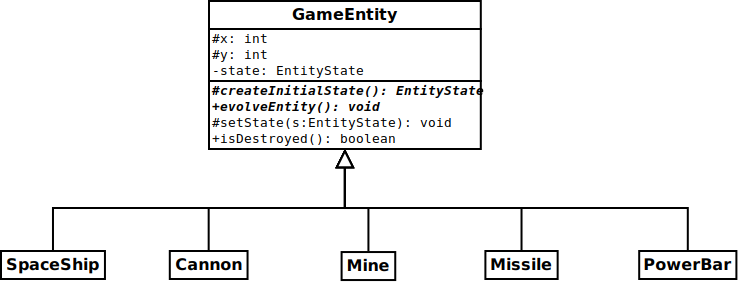
\includegraphics[width=15cm]{GameEntity.pdf}
\caption{Diagramma UML della classe \textsf{GameEntity}}
\label{img:GameEntity}
\end{figure}

Presentiamo nel dettaglio i vari pattern utilizzati.

\subsection{Utilizzo dal pattern \emph{State}}

Al fine di modellare al meglio la necessit\`a di mantenere uno stato e di evolverlo da parte delle \textsf{GameEntity} si \`e utilizzato il pattern \emph{State}: \`e stata definita la classe astratta \textsf{EntityState} che rappresenta un generico stato di un'entit\`a.

Ogni classe provveder\`a a realizzare le sottoclassi di \textsf{EntityState} e a fornire l'implementazione dei metodi astratti della classe.

\begin{figure}[h]
\centering
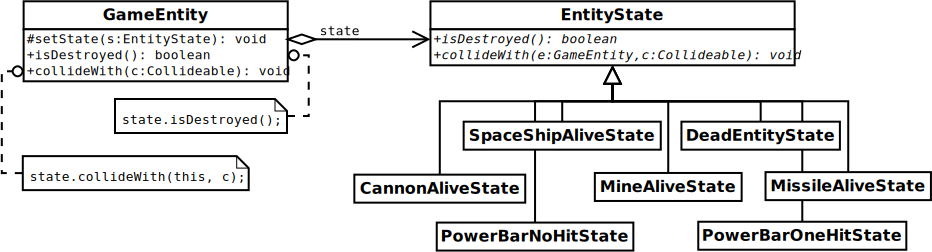
\includegraphics[width=15cm]{State.pdf}
\caption{Diagramma UML del pattern \emph{State}}
\label{img:State}
\end{figure}

Nel diagramma in figura \ref{img:State} si nota che la classe \textsf{EntityState} contiene i metodi: \textsf{isDestroyed} per verificare se l'astronave si trova in uno stato in cui \`e stata distrutta, e \textsf{collideWith} per gestire la collisione fra 


\section{Gestione delle collisioni}
\label{sec:collisioni}

\section{Gestione dei comandi}
\label{sec:comandi}

\section{Avvio e terminazione del gioco}
\label{sec:avvio}

\section{Gestione del multiplayer}
\label{sec:multiplayer}

\section{User guide}
\label{sec:guide}

La simulazione \`e stata realizzata in Java utilizzando il simulatore Peersim ed \`e stata corredata di un file \textbf{ant} (il file \texttt{build.xml}) che offre dei target per automatizzare il processo di compilazione e di esecuzione del software.

Per funzionare, la simulazione ha bisogno di un file di configurazione in input da cui poter caricare la configurazione della rete (numero di nodi, numero di link, protocolli da utilizzare, etc...). Alcuni esempi di file di configurazione possono essere trovati all'interno della cartella \texttt{example/}.

Per compilare la simulazione \`e necessario posizionarsi all'interno della directory dove \`e contenuto il software ed invocare da terminale il comando

\begin{lstlisting}[basicstyle=\ttfamily]
ant build
\end{lstlisting}

che provveder\`a ad invocare il compilatore \texttt{javac} per compilare i sorgenti presenti all'interno della cartella \texttt{src/}, i file \texttt{.class} generati si troveranno all'interno della cartella \texttt{bin/}. 

Per pulire la cartella \texttt{bin/} al fine di avere un ambiente pulito per poter effettuare una nuova compilazione \`e possibile utilizzare il target
\begin{lstlisting}[basicstyle=\ttfamily]
ant clean
\end{lstlisting}

\`E infine possibile generare un file \texttt{jar} contenente tutti i file compilati e tutte le librerie necessarie all'esecuzione. Per farlo \`e sufficiente invocare il target
\begin{lstlisting}[basicstyle=\ttfamily]
ant jar
\end{lstlisting}
Verr\`a generato un file chiamato \texttt{p2p\_final.jar} all'interno della cartella principale del software.
Per avviare il file \texttt{jar} \`e necessario invocare il comando
\begin{lstlisting}[basicstyle=\ttfamily]
java -jar p2p_final.jar [file di configurazione]
\end{lstlisting}

\subsection{Documentazione}

Al fine di rendere il codice sorgente pi\`u comprensibile, il software \`e stato corredato di documentazione. In particolare tutte le parti del codice sorgente che potrebbero risultare di difficile comprensione sono state commentate. Inoltre ogni funzione e classe del software \`e stata documentata con il formato \textsf {javadoc}, la documentazione generata pu\`o essere visionata all'interno della cartella \textsf{doc/} e pu\`o essere rigenerata utilizzando il comando
\begin{lstlisting}[basicstyle=\ttfamily]
ant javadoc
\end{lstlisting}

Per una comprensione organica del software si consiglia la lettura della seguente relazione nella sua interezza. La presente relazione viene rilasciata in Pdf ed in \LaTeX\ e pu\`o essere visionata all'interno della cartella \texttt{doc/tex/}.

\subsection{Avvio della simulazione}

Una volta compilato il software \`e possibile invocarlo tramite il comando
\begin{lstlisting}[basicstyle=\ttfamily]
ant Execute [-Dfile=nomefile]
\end{lstlisting}

Con \texttt{-Dfile=nomefile} \`e possibile impostare il file di configurazione da usare. Per effettuare alcune computazioni di esempio \`e quindi sufficiente impostare \texttt{-Dfile=example/<nomefile.conf>}, eseguendo alcuni dei files di esempio gi\`a predisposti all'interno della cartella \texttt{example}.

I nomi dei files contenuti nella cartella \texttt{example} permettono di comprendere facilmente quali sono le configurazioni impostate. Sono stati predisposti calcoli solamente \textsc{count} oppure \textsc{count-beacon}, con grafi random, small-world e scale-free. Inoltre sono stati predisposti esempi con debugger attivato ed altri esempi in cui si calcolano altre funzioni (massimo, somma, etc...).

Se la struttura dei file di configurazione non fosse chiara \`e possibile visionare il file \textsf{example.conf} che contiene tutti i commenti necessari a comprendere le impostazioni possibili.

\end{document}
